\documentclass{article}
\usepackage[utf8]{inputenc}
\usepackage[polish]{babel}
\usepackage[T1]{fontenc}
\usepackage{multicol}
\usepackage{multirow}
\usepackage{amsmath}
\usepackage[export]{adjustbox} 
\usepackage{float}
\usepackage{graphicx}
\usepackage{chngpage}
\usepackage{longtable}
% table struts
\usepackage{listings}
\usepackage{layout}

\usepackage{caption}
\usepackage{rotating}
\usepackage{geometry}
%  \usepackage{draftwatermark}
%\SetWatermarkText{DRAFT}
%\SetWatermarkScale{5}
\usepackage{lscape}
\newcommand\T{\rule{0pt}{2.6ex}}       % Top strut
\newcommand\B{\rule[-1.2ex]{0pt}{0pt}} % Bottom strut
\usepackage{array}   % for \newcolumntype macro
\newcolumntype{L}{>{$}l<{$}} 
\begin{document}
	
	\begin{titlepage}
		
		
		
		\vspace{5cm}
		
		\begin{center}
			\vspace*{1cm}
			
			{\Huge \textbf{Optymalne sterowanie warunkiem brzegowym z wykorzystaniem metody Adjoint}}
			
			\vspace{0.5cm}
			{\huge Projekt 13}
			
			\vspace{1.5cm}
			\large{Filip Hahs}
			
			
		\end{center}
		\vfill
		
		
	\end{titlepage}
	\section{Problem}
Celem projektu było napisanie programu znajdującego taki rozkład temperatury zewnętrznej na brzegu $\Gamma_2$ w każdej chwili, aby rozkład temperatury w przestrzeni $\Omega$ był maksymalnie jednorodny. Na krawędziach należących do $\Gamma_1$ zadany jest adiabatyczny warunek brzegowy. 
\begin{figure}[H]
	\centering
	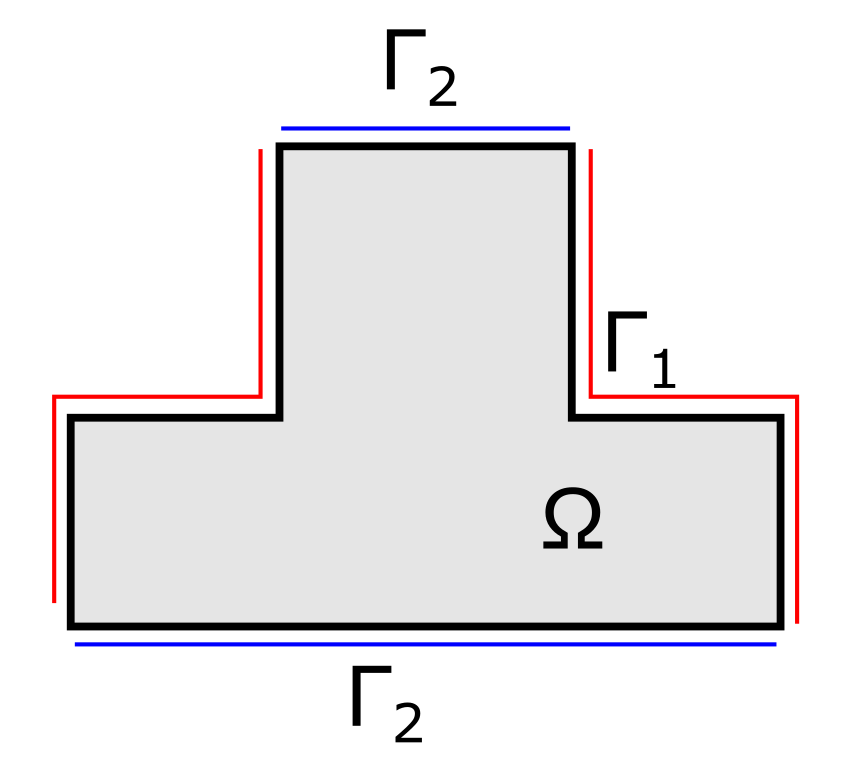
\includegraphics[width=0.5\linewidth]{plyta}
	\caption{Przestrzeń obliczeniowa}
	\label{fig:plyta}
\end{figure}
Równanie różniczkowe cząstkowe ma postać:
\begin{align*}
	\begin{cases}
		\frac{\partial u}{\partial t} = D\Delta u\; \text{dla}\; u\in\Omega\\
		D\frac{du}{dn} = \beta(c-u) \; \text{dla}\; u\in\Gamma_2\\
		\frac{du}{dn} = 0 \; \text{dla}\; u\in\Gamma_1\\
	\end{cases}
\end{align*}
gdzie:
\begin{align*}
	&D \text{ - to dyfuzyjność (przewodność cieplna)}\\
	&\beta \text{ - to współczynnik przyjmowania ciepła na brzegu}\\
	&c \text{ - to temperatura zewnętrzna, czyli zmienna sterowana}
\end{align*}.
W chwili początkowej:
\begin{align*}
	u(x,y, 0) = u_0(x,y)
\end{align*}
Program ma zadanie minimalizować funkcję celu, zadaną wzorem:
\begin{align*}
	J=\int_{\Omega}[u(\textbf{x},T)-V]^2d\Omega
\end{align*}
gdzie $V$ to zadana wartość średniej temperatury, $T$ to koniec przedziału czasowego a \textbf{x} to położenie wewnątrz domeny.
\section{Wprowadzenie teoretyczne}
Metoda "adjoint", czyli gradientu sprzężonego polega na znalezieniu funkcji $u_*$, która reprezentuje wpływ sterowania na wartość funkcji celu. Aby znaleźć tą funkcję wyprowadzono potencjał rozszerzony:
\begin{align*}
	\hat{J} = \int_{\Omega}[u(\textbf{x},T)-V]^2d\Omega + \int_{0}^{T}\int_\Omega(	\frac{\partial u}{\partial t}-D\Delta u)u_* d\Omega dt
\end{align*}
Na tym etapie $u_*$ jest dowolną funkcją. Kolejnym krokiem jest wykorzystanie rachunku wariacyjnego, aby obliczyć wariancję funkcjonału rozszerzonego ze względu na mała zmianę rozwiązania $\delta u$, czyli przyrost $\hat{J}(u+\delta u) - \hat{J}(u)$
\begin{align*}
	\delta\hat{J} = \int_{\Omega}[u(T)-V]\delta u(T)d\Omega + \int_{0}^T\int_{\Omega}(	\frac{\partial u}{\partial t}-D\Delta u)u_*d\Omega dt
\end{align*}
Następnie, skorzystano z drugiego twierdzenia Greena, aby uwolnić  $\delta u$ od różniczkowania.
\begin{align*}
	\int_{\Omega}\Delta\delta u\cdot u_* - \int_{\Omega}\Delta u_*\cdot\delta u\delta\Omega &= \int_{\partial\Omega}\frac{d}{dn}(\delta u)u_* dS-\int_{\partial\Omega}\frac{d}{dn}u_*\delta u dS\\
	&\Big\Downarrow\\
	=\int_{\Omega}\Delta\delta u \cdot u_* d\Omega = \int_{\Omega}\Delta u_*\cdot \delta u d \Omega &+ \int_{\partial\Omega}\delta(\frac{du}{dn})u_* dS - \int_{\partial\Omega}\frac{du_*}{dn}\delta u dS=\\
	=\int_{\Omega}\Delta u_*\cdot \delta u d\Omega &+ \int_{\Gamma_2}\frac{\beta}{D}(\delta c - \delta u)u_*dS - \int_{\partial\Omega}\frac{du_*}{\partial n}\delta u dS
\end{align*}
Następnie zastosowano przekształcenie:
\begin{align*}
	\int_{0}^{T}\int_{\Omega}\partial_t\delta u \cdot u_* d\Omega dt = \int_{\Omega}[\int_{0}^{T}\partial_t(u_*\delta u)dt - \int_{0}^{T}\partial_t u_* \delta u dt]=\\
	=\int_{\Omega}[u_*(T)\delta u(T)-u_*(0)\delta u(0)]d\Omega + \int_{0}^{T}\int_{\Omega}(-\partial_t u_*)\delta u d\Omega dt
\end{align*}
Następnie podstawiono:
\begin{align*}
	\delta \hat{J} =& \int_{0}^{T}\int_{\Omega}[-\partial_t u_*-D\Delta u_*]\delta u d\Omega dt - \int_{0}^{T}\int_{\Gamma_2}\beta u_*\delta c dSdt- \\
	&-\int_{0}^{T}\int_{\Gamma_2}(\frac{du_*}{dn}+\beta u_x)\delta u dSdt - \int_{0}^{T}\int_{\Gamma_1}\frac{du_*}{dn}\delta u dSdt+\\
	&+ \int_{\Omega}[u_*(T)+u(T)-V]\delta u(T)d\Omega
\end{align*}
Następnie wybrano funkcję $u_*$, tak aby wyrażenie na $\delta\hat{J}$ nie zawierało wyrażeń $\delta u \;\text{i}\; \delta u(T)$. Zrobiono tak, aby obliczenie $\hat{J}$ wymagało jedynie obliczenia $\delta c$. Jest to podstawowa idea metody gradientów sprzężonych.
Funkcja $u_*$ ma postać:
\begin{align*}
	\begin{cases}
		-\partial_t u_* = D\Delta u_* \;\text{w}\; \Omega \\
		\frac{du_*}{dn} + \beta u_* = 0 \; \text{na} \; \Gamma_2\\
		\frac{du_*}{dn} = 0 \; \text{na} \; \Gamma_1\\
	\end{cases}
\end{align*}
Funkcja ta ma warunek \textbf{końcowy}:
\begin{align*}
	u_*(T) = V - u(T)
\end{align*}
Całkowanie funkcji $u_*$ odbywa się \textbf{wstecz w czasie}.
Po obliczeniu $u_*(T)$ w $\Omega$ na przedziale $[0, T]$ można wyznaczyć:
\begin{align*}
	\frac{D\hat{J}}{Dc} = -\beta u_*
\end{align*}
\section{Implementacja programu}
\subsection{Ogólny schemat programu}
Na poniższym schemacie przedstawiono działanie programu "z lotu ptaka", przedstawiając ogólny przepływ danych. $\epsilon$ oznacza małą, dodatnią liczbę.
\begin{figure}[H]
	\centering
	\includegraphics[width = 0.55\textwidth]{main_chart.png}
\end{figure}
\subsection{Dyskretyzacja przestrzeni}
W programmie wykorzystano równomiernie rozłożoną siatkę różnicową.
\end{document}